\documentclass[12pt]{article}
\usepackage{graphicx}
\usepackage{titlesec}
\usepackage{xlop}
\usepackage{url}
\usepackage{subcaption}
\usepackage{geometry}
\graphicspath{ {./images/} }
\usepackage[fleqn]{amsmath}
\usepackage{tikz}
\usepackage{listings}
\usepackage{karnaugh-map}
\geometry{
    a4paper, 
    top=20mm,
    left=20mm,
}
\setlength{\parindent}{4em}
\setlength{\parskip}{1em}
\renewcommand{\baselinestretch}{1.5}

\title{Final Project: ES4 Spring 2021}
\date{5/11/2021}
\author{Ibrahima Barry, WIlly Lin \\ Zach Osman, James Eidson \\ ECE Tufts University}

\titleformat{\section}
    {\normalfont\Large\bfseries}{\thesection}{1em}{}[{\titlerule[1pt]}]

\lstdefinestyle{myListingStyle} 
    {
        basicstyle = \small\ttfamily,
        breaklines = true,
    }

\begin{document}

\maketitle

\begin{flushleft}

\section{Overview}
\begin{center}
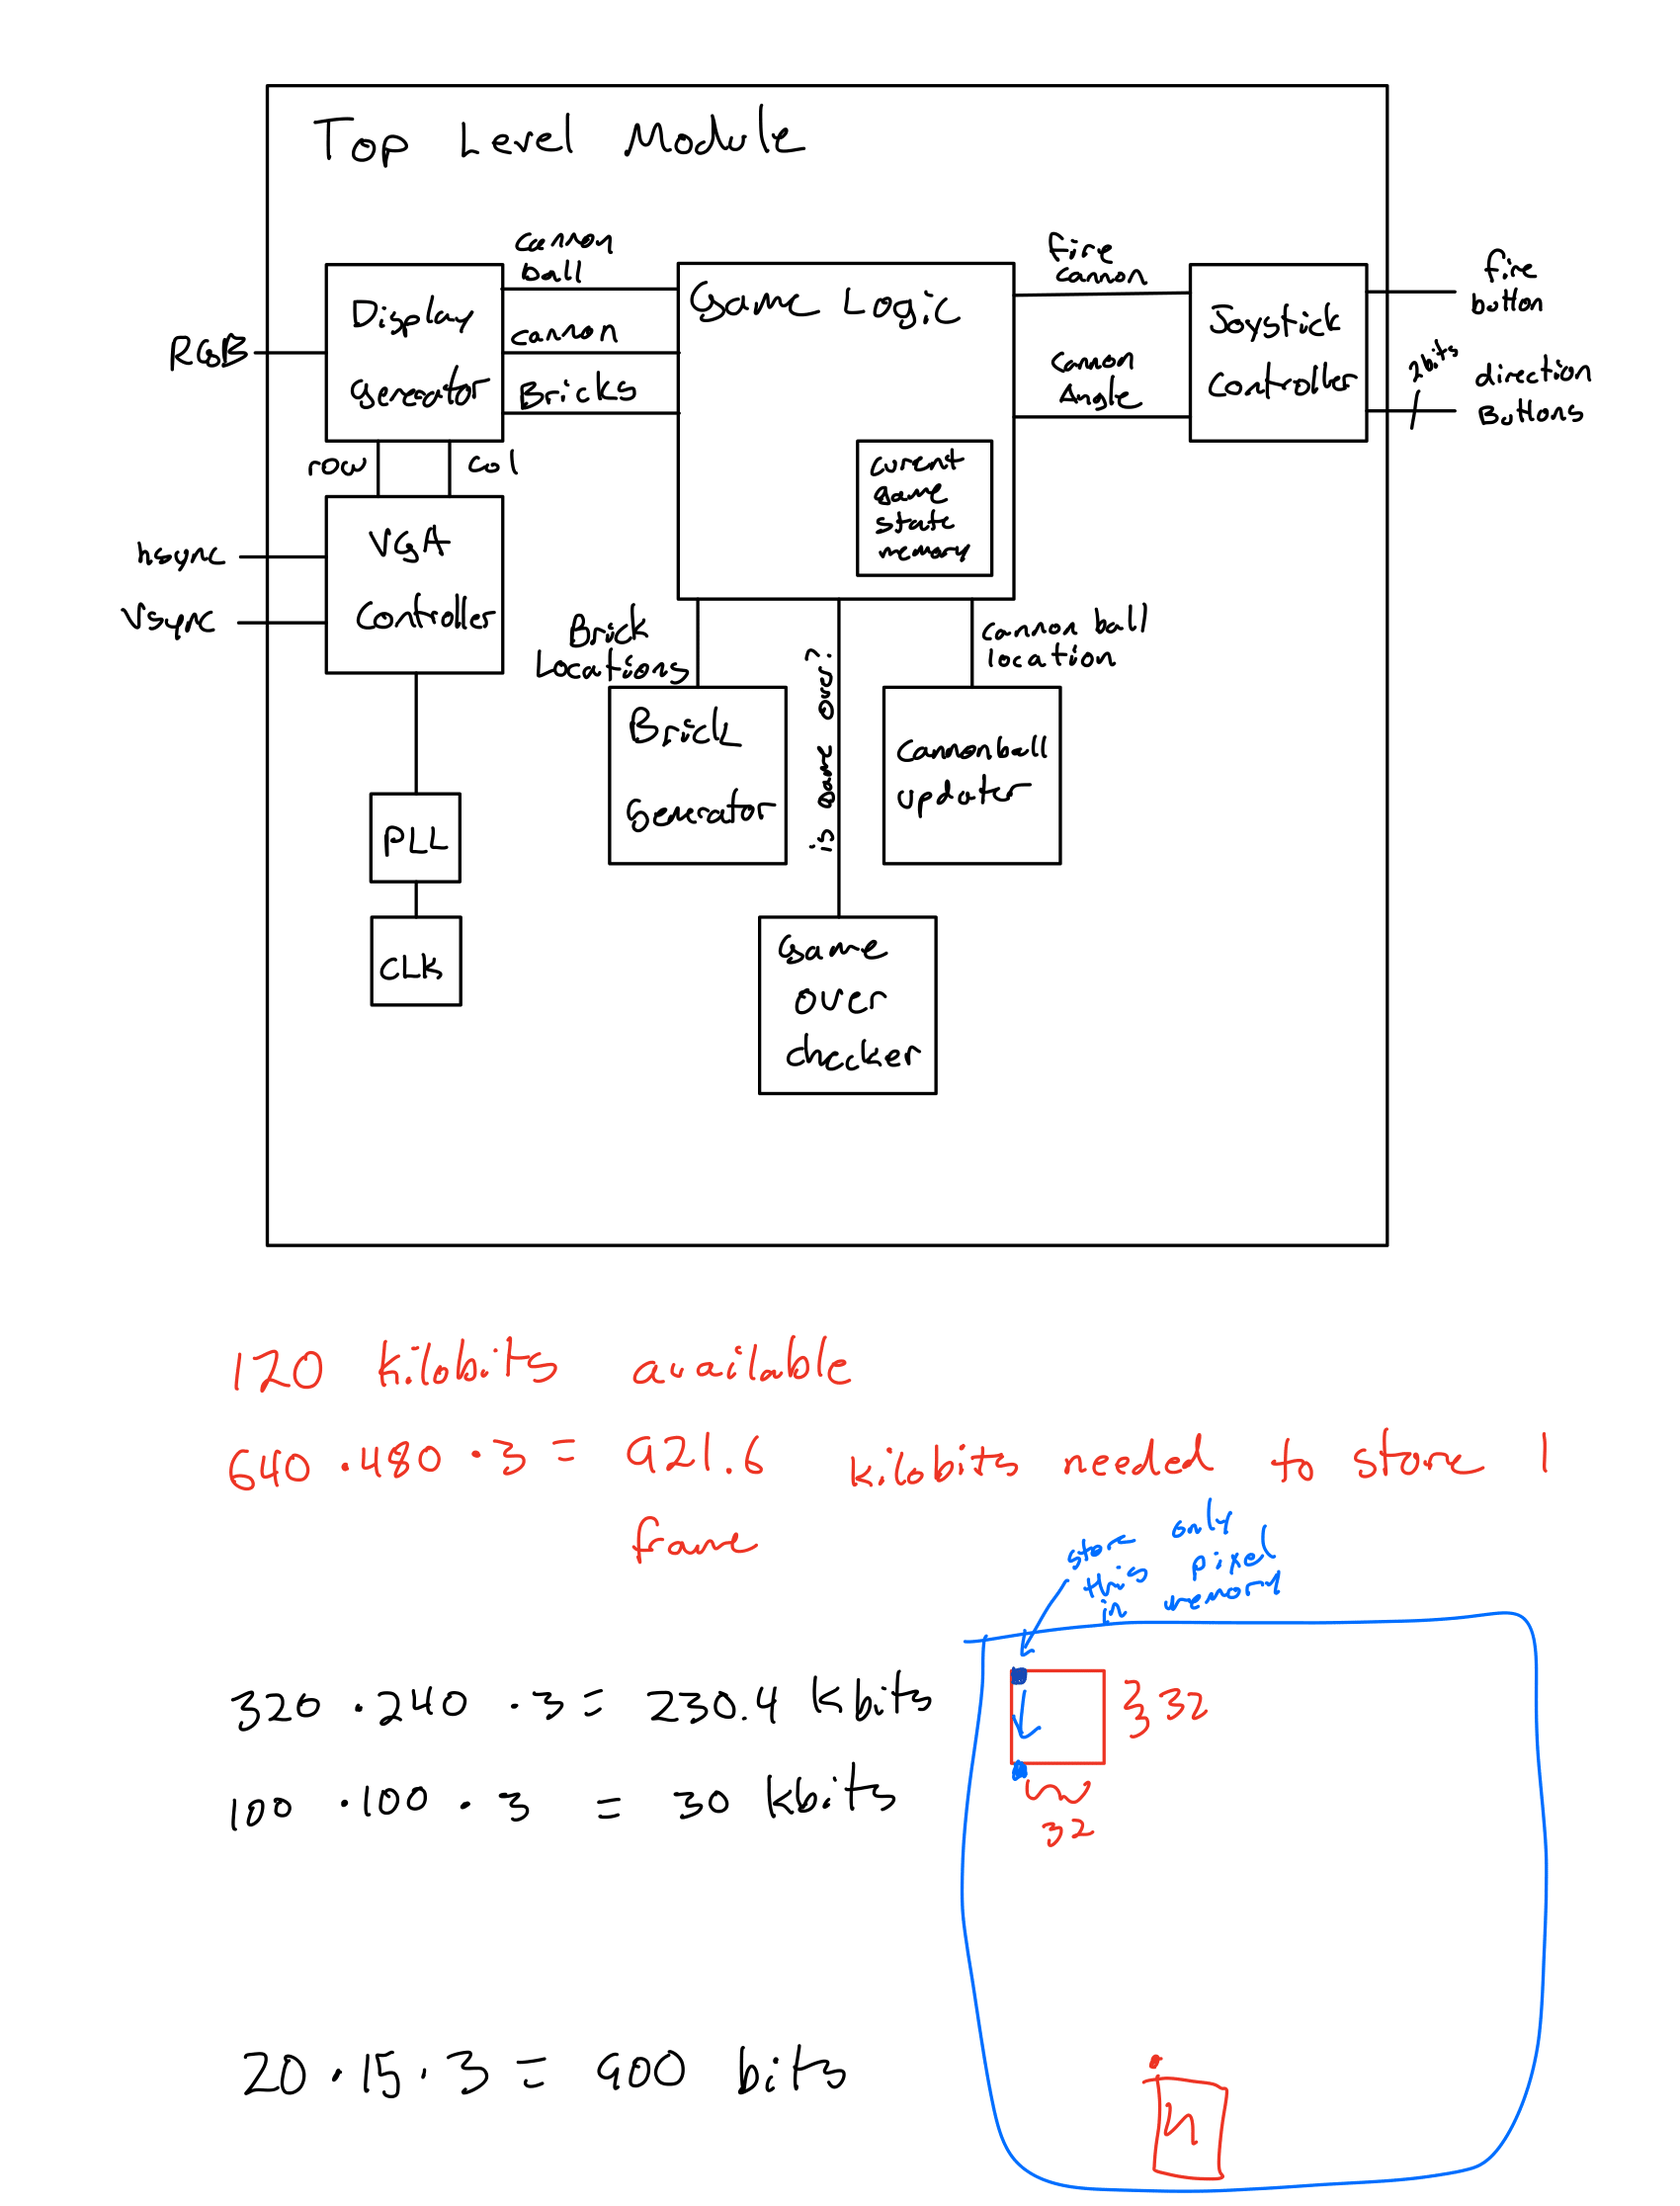
\includegraphics[width=10cm, height=10cm]{blockDiagram}
\end{center}
This game is a variation of the game brickBreaker where the player fires a
cannonball out of a cannon and works to destroy the bricks that are displayed on
the screen. There are three main parts to this project: displays, controls, and
game logic. 'Displays' were done using a VGA, 'controls' were done by using
an NES gamepad, and 'game logic' done in the 'top' module of our project. 
VGA sends the current row and column to display on the screen. The NES gamepad
takes data in the form of buttons pressed and stores it in a shift-register. A
clock is driven for 8 cycles (the number of buttons is 8) and the data signal is
synchronized with the clock. When a button is pressed the corresponding bit of
the output of the register is set to low. The top module controls the general
logic of the game such as drawing the bricks and the cannnon. Top also controls
the memory usage of the game. Overall, objects are drawn in the top module,
displayed via the display module, and those objects are then controlled via the
cannon module (which is connected to the gamepad). 

\section{Technical Description and Design}
\subsection{Top Module}

The top module is where the main game logic is handled. It's inputs are the
12MHz clock of the FPGA and the data from the the controller. It outputs the
necessary signals for the controller and the VGA to work. It's components
are the pll, vga, display, and cannon. The main function of top is to draw the
game objects. This the code to draw the bricks:\\
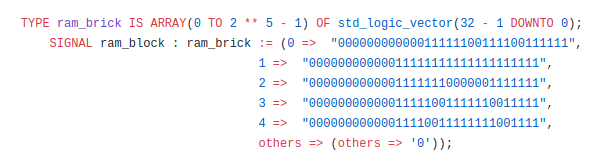
\includegraphics[width=15cm, height=5cm]{drawingBricks}

Where there is a '1' bit is where a brick is drawn. The other details are more
complicated but in general $'1' = $ brick drawn $'0'=$ brick not drawn. $0 - 4$
represent the row being drawin. One of the major challenges encountered here was
figuring out how to destroy a brick when it is hit by a cannon. This means where
there is a $'1'$ bit, meaning a block is drawn at that position, we have to invert
the bit when it is hit by the ball. The display module now knows not to draw
that brick. This was solved by using bit-masking to change the bit.\\ 
eg) consider the row of bricks: $00000000000011111100111100111111$
suppose the block at index 31 needs to be destroyed then the $XOR$ logical
operatoin works well for this. 
$00000000000011111100111100111111 \oplus 00000000000000000000000000000010 =
00000000000011111100111100111101$ 

We create a new bit word of the same size as the ram block  with the corresponding bit we want destroyed to be '1'
and the other bits to '0'. Then $ 1 \oplus 1 = 0$ so this will invert the bit we
want inverted. The other bits are unchanged as $1 \oplus 0 = 1$ and $0 \oplus 0 = 0$.  

\subsection{Cannon Control Module}
This is where the NES gamepad is used to control our game objects: the cannon
and the cannon ball. Cannon sends it's data signal (which is also in the top
module) to the NES controller and outputs the ball and cannon position based on
the which button is pressed. Instead of using all 8 bits of the output of the
NES only three were used the left and right button to move the cannon
horizontally and the "A" button to fire the cannon ball. The rest of the bits
were sent to 0. \\
The logic for moving the cannon was relatively simple: if the button is pressed
(the signal is low) change the cannon's position by 1 to the left or right (which is later used in the top
and display modules in order to actually display the change). If the fire button
is pressed: change the row the ball is displayed (move the ball up) else set the
column of the ball to the cannon's colum and it's row to the cannon's row as
well. \\

The biggest challenge we had was figuring out how to smoothly fire the cannon
ball. The firing was happening too rapidly, pressing the button jumped the ball
too far up the screen. The solution we came up with was to have the ball
continously be where the cannonis and if the user presses the fire button the
ball goes up and stops once the user stops pressing the button. THe ball shot
4-24 times based on how long the button was held. 
\section{Results and Testing}

\section{Debugging Log}

\section{Reflection} 

\section{Work Divison} 

\section{source code}
%Add link to the github


\end{flushleft}
\end{document}
